% Chapter 1

\chapter{Introducción general} % Main chapter title

\label{Chapter1} % For referencing the chapter elsewhere, use \ref{Chapter1} 
\label{IntroGeneral}

En este capítulo se introduce la problemática y se interpreta la importancia que
implica el trabajo. Luego, se realiza un análisis del estado de arte sobre la ges-
tión eficiente de salud de cultivos y se puntualizan los objetivos y el alcance del
trabajo.

%----------------------------------------------------------------------------------------

% Define some commands to keep the formatting separated from the content 
\newcommand{\keyword}[1]{\textbf{#1}}
\newcommand{\tabhead}[1]{\textbf{#1}}
\newcommand{\code}[1]{\texttt{#1}}
\newcommand{\file}[1]{\texttt{\bfseries#1}}
\newcommand{\option}[1]{\texttt{\itshape#1}}
\newcommand{\grados}{$^{\circ}$}

%----------------------------------------------------------------------------------------

%\section{Introducción}

%----------------------------------------------------------------------------------------
\section{Contexto del trabajo}

En la EEA San Pedro de INTA se busca intensificar de manera sustentable la producción
de frutales, hortalizas y viveros. Actualmente, la inspección y evaluación
dependen de visitas de campo y observaciones manuales, procesos costosos, laboriosos
 y con alcance limitado. Además, el cambio climático y la variabilidad
meteorológica añaden capas adicionales de complejidad la gestión agronómica.

El Laboratorio de Biotecnología cuenta con datos históricos sobre las etapas de
floración y maduración de frutos en durazneros. En este contexto, las imágenes
satelitales se presentan como una herramienta poderosa, ya que ofrecen datos
consistentes y de amplia cobertura, permiten evaluar la vegetación de forma
precisa y objetiva mediante índices especializados.

En la figura \ref{fig:diagramatesis} se ilustra el flujo de información y el esquema de entrenamiento 
previsto para este trabajo.

\begin{figure}[h]
	\centering
	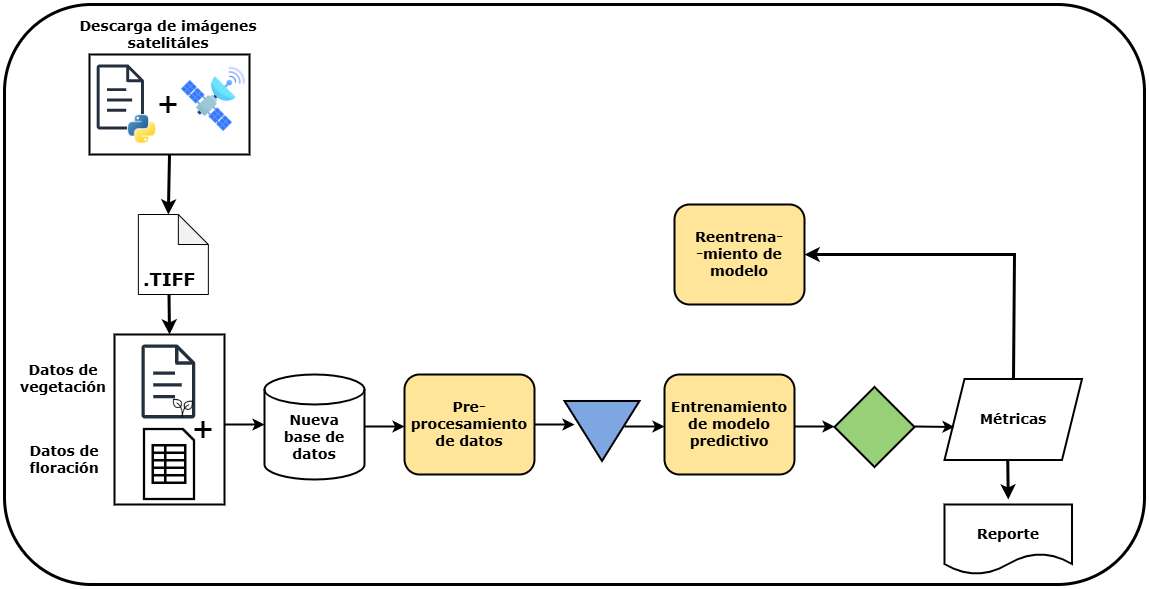
\includegraphics[width=\textwidth]{./Figures/flujo_tesis_tffa.png}
	\caption{Diagrama de flujo del proceso de entrenamiento predictivo.}
	\label{fig:diagramatesis}
\end{figure}


El propósito de este trabajo es automatizar la gestión de montes frutales mediante el 
uso de datos disponibles e índices obtenidos de imágenes satelitales. Para lograr este
objetivo, se hará uso de métodos de aprendizaje automático, aprendizaje profundo y 
técnicas de preprocesamiento de datos. Se propone una herramienta accesible para los 
usuarios, que optimiza los resultados y reduce el tiempo y esfuerzo requeridos.

\section{Estado del arte}

En los últimos años, la recopilación masiva de datos agrícolas ha transformado la 
toma de decisiones en la gestión de cultivos, lo que ha permitido optimizar su salud
y rendimiento. Al mismo tiempo, el aprendizaje profundo se ha consolidado como una
herramienta popular en múltiples áreas de investigación, debido a su capacidad para
procesar grandes volúmenes de información provenientes de diversas fuentes. En 
este contexto, las imágenes satelitales ocupan un papel crucial, ya que su 
disponibilidad sin precedentes ha impulsado el avance de la investigación en teledetección.

La caracterización de montes frutales mediante imágenes satelitales ha 
experimentado avances significativos, con estudios que exploran técnicas y
tecnologías para mejorar la identificación y supervisión de estos cultivos.
Diversas investigaciones han desarrollado metodologías que integran sensores 
remotos y algoritmos de aprendizaje automático para analizar el estado de la 
vegetación, detectar factores de estrés y prever el rendimiento de las cosechas. 
Estas soluciones no invasivas permiten obtener información detallada sin afectar
las condiciones del terreno, representando un enfoque eficiente y escalable 
para el manejo agrícola.

Los avances en teledetección han revolucionado la supervisión de huertos frutales, 
al proporcionar herramientas innovadoras que permiten evaluar la salud de los cultivos
y optimizar su gestión. La integración de imágenes satelitales con modelos predictivos
ha posibilitado la automatización del monitoreo, lo que mejora la precisión en la 
detección de anomalías y facilita la toma de decisiones basada en datos. Estas
tecnologías no solo permiten reducir los costos operativos, sino que también 
promueven una producción agrícola más sostenible, y posicionan a la teledetección 
como una herramienta esencial en la agricultura de precisión.

\subsection{Avances recientes}

\begin{itemize}
  \item El trabajo titulado \textit{Segmentación multiescala orientada a objetos y método basado en la 
  fusión de múltiples características para la identificación de árboles frutales típicos en 
  regiones áridas mediante imágenes de satélite Sentinel 1 y 2} evaluó la aplicabilidad de datos temporales
  de los satélites Sentinel-1/2 para la clasificación de árboles frutales en la
  cuenca del Tarim, China. Para ello, se emplearon técnicas de segmentación multiescala y fusión de
  múltiples características para extraer con precisión las especies de árboles
  frutales \citep{Liang2024}.
  \item Otro estudio utilizó imágenes de alta resolución obtenidas por 
  vehículos aéreos no tripulados para extraer información detallada sobre 
  árboles individuales en huertos, resaltando la importancia de métodos eficientes
  y confiables en la gestión de huertos \citep{Dong2020}.
  \item Diversas investigaciones han integrado datos de sensores multiespectrales y 
  térmicos con algoritmos de aprendizaje automático, con el fin de monitorear la salud 
  de los cultivos y detectar factores de estrés en huertos frutales \citep{Kumar}.
  \item Se han desarrollado sistemas que integran sensores montados en tractores con 
  plataformas de software basadas en inteligencia artificial. Estas soluciones permiten recopilar datos 
  precisos sobre cada árbol, lo que facilita una gestión más eficiente y reduce la 
  dependencia de mano de obra \cite{OrchardRobotics2024}.
\end{itemize}

\subsection{Aprendizaje automático aplicado a la salud de cultivos}

La aplicación de modelos de aprendizaje automático en la caracterización de 
montes frutales de durazno mediante imágenes satelitales ha avanzado 
notablemente en los últimos años.

A continuación, se presentan algunas investigaciones actuales: 
\begin{itemize}
  \item Un estudio evaluó la capacidad de algoritmos como Extreme Gradient Boosting (XGBoost),
   Random Forest (RF) y Support Vector Regressor (SVR) para predecir parámetros ecofisiológicos en un huerto de
   duraznos ubicado en una región semiárida. Para este fin, se utilizaron datos multiespectrales obtenidos por satélite.
   El modelo Random Forest funcionó mejor para predecir la asimilación neta, mientras que el SVR fue más preciso con otros indicadores 
   fisiológicos de la planta. Estos hallazgos subrayan el potencial de integrar técnicas de aprendizaje automático 
   con imágenes satelitales de alta resolución para monitorear la salud de los cultivos y optimizar las prácticas
   de riego \citep{Campi2024}.
  \item Una contribución reciente ha explorado el uso de redes neuronales profundas para la detección de frutos en huertos.
   Un estudio comparó los modelos YOLOv8 y Mask R-CNN en la segmentación de objetos en entornos complejos de huertos. Los resultados indicaron que
   YOLOv8 superó a Mask R-CNN en precisión y tiempo de inferencia; obtuvo un 90\,\% de precisión y un 95\,\% de recall  
   en la detección de múltiples clases. Estos resultados destacan la eficacia de los modelos de una sola etapa como YOLOv8 para 
   aplicaciones en agricultura de precisión, que facilitan tareas como la cosecha selectiva y la poda precisa \citep{Sapkota2023}.
  \item Un trabajo reciente exploró la clasificación de variedades de durazno en huertos a partir de imágenes hiperespectrales, en combinación 
  con algoritmos de aprendizaje automático. Los autores evaluaron modelos como Support Vector Machine (SVM), Random Forest (RF) 
  y k-Nearest Neighbors (k-NN) para diferenciar cultivares basándose en firmas espectrales. Los resultados mostraron que el modelo 
  SVM logró la mayor precisión con el 90\,\% en la identificación de variedades específicas. La investigación pone en evidencia el valor 
  de los datos espectrales detallados combinados con técnicas de machine learning. El uso de esta información permite caracterizar con 
  precisión el cultivo, facilitar un manejo agronómico diferenciado y respaldar la toma de decisiones basadas en datos \citep{Zhou2022}.
\end{itemize}


\section{Alcance y Objetivos}
El objetivo principal del trabajo consistió en desarrollar un algoritmo que permita descargar y analizar 
imágenes satelitales, con el fin de vincularlas a características específicas de durazneros. Específicamente, 
determinar, a partir de los datos disponibles, el progreso de las etapas de floración y maduración de 
los frutos en los árboles.

\subsection{Alcance del proyecto}
A continuación, se detallan las actividades incluidas en este trabajo:

\begin{itemize}
  \item Evaluación de las diferentes fuentes de datos disponibles:
  \begin{itemize}
    \item Datos tabulares, que corresponden a mediciones de campo
    de las etapas de floración y maduración de frutos, obtenidos durante 5
    años.
    \item Imágenes satelitales, correspondientes a los lotes de durazneros monitoreados.
    \end{itemize}
  \item La determinación del progreso de las etapas de floración y maduración de
  los frutos en el duraznero.
  \item El desarrollo de una herramienta de fácil acceso para el equipo del cliente.
  \item La elaboración de un informe que detalle el procedimiento realizado y los resultados obtenidos.  
  \end{itemize}

  Los siguientes elementos quedan fuera del alcance del presente trabajo:
  \begin{itemize}
    \item El desarrollo de una interfaz web para el sistema.
    \item El despliegue del desarrollo en un entorno de producción.
    \end{itemize}

